% !TeX root = ../main.tex
\documentclass[./../main.tex]{subfiles}

\begin{document}

Đối với hệ thống có nhiều role người dùng thì phần giao diện đóng một vai trò vô cùng quan trọng trong trải nghiệm của người sử dụng. Các màn hình của mỗi role phải được thiết kế dựa trên vai trò, nhu cầu của từng nhóm người dùng theo cách đơn giản hóa nhưng vẫn chung một phong cách và truyền tải được đến người dùng những nội dung quan trọng của trang web.

\subsection{Màu sắc}
Toàn bộ hệ thống được thiết kế dựa trên tông màu xanh nổi bật xuất hiện ở các nút bấm, các hình ảnh minh họa, các tiêu đề được chọn,... đem lại trải nghiệm đồng nhất cho toàn bộ trang web:

\begin{figure}[H]
	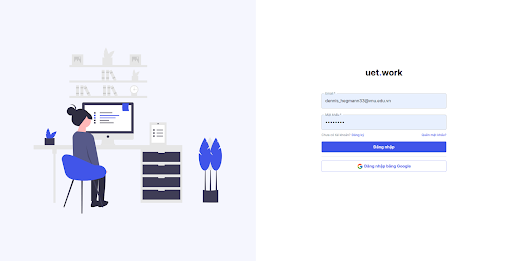
\includegraphics[width=\linewidth]{./images/image31.png}
	\caption{Ví dụ về màu sắc được sử dụng trong hệ thống}
	\label{fig:example_color}
\end{figure}

\subsection{Đa ngôn ngữ}

Với mục đích mở rộng hệ thống cho các Khoa, các tổ chức có sinh viên quốc tế, phần giao diện của trang web có hỗ trợ đa ngôn ngữ, hiện tại là Tiếng Việt và Tiếng Anh.

\begin{figure}[H]
	
\includegraphics[width=\linewidth]{./images/image30.png}
	\caption{Ví dụ về việc lựa chọn ngôn ngữ hiển thị}
	\label{fig:multiple_lang}
\end{figure}

Bằng việc sử dụng framework i18n, việc mở rộng thêm các ngôn ngữ khác là vô cùng đơn giản. Các file dịch đều để dưới dạng json rất rõ ràng như hình \ref{fig:example_i18n}, khi muốn thêm hoặc chỉnh sửa bản dịch của một ngôn ngữ, chỉ cần vào file dịch của ngôn ngữ đó để tạo mới hoặc chỉnh sửa.

\begin{figure}[H]
	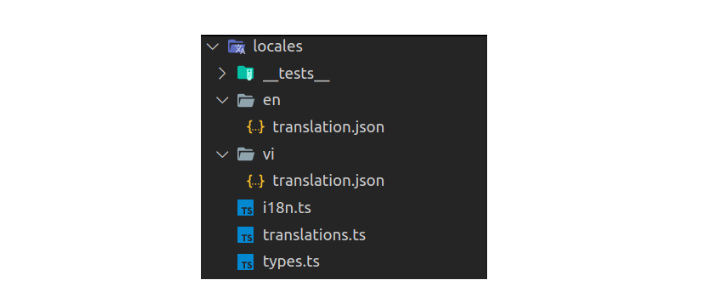
\includegraphics[width=\linewidth, scale=0.5]{./images/image86.png}
	\caption{Cách tổ chức file dịch của các ngôn ngữ}
	\label{fig:example_i18n}
\end{figure}

\subsection{Tăng trải nghiệm người dùng}

Để người dùng có trải nghiệm tốt hơn khi sử dụng ứng dụng, không cảm thấy nhàm chán khi đợi tải trang, hệ thống hiển thị màn hình loading sinh động trong khi đang tải.

\begin{figure}[H]
	
\includegraphics[width=\linewidth]{./images/image32.png}
	\caption{Ví dụ về màn hình loading}
	\label{fig:example_loading}
\end{figure}

\subsection{Áp dụng nguyên lý thiết kế giao diện}

Giao diện của các màn hình được thiết kế dựa theo 5 nguyên lý thiết kế giao diện người dùng: tính cân bằng (balanced), sự nhịp điệu (rhythm), sự hài hòa (harmony), sự thống trị (dominance), sự căn chỉnh (alignment).

Tính cân bằng và nhịp điệu được thể hiện thông qua việc phân chia giao diện thành các khối, sắp xếp vị trí của chúng cũng như các khoảng trống micro, macro một cách hợp lý và sau cùng là lặp lại đều đặn các phần tử có cùng chức năng.

\begin{figure}[H]
	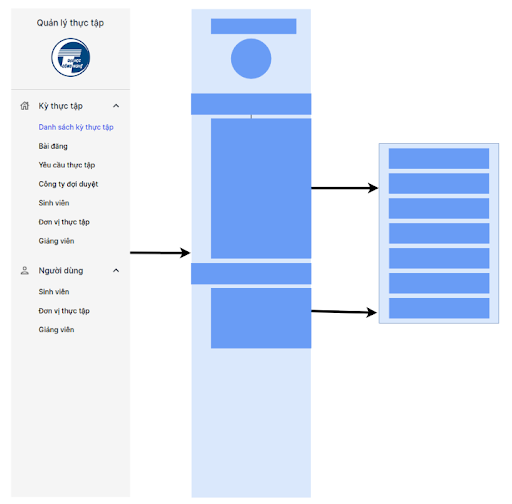
\includegraphics[width=\linewidth]{./images/image33.png}
	\caption{Ví dụ Nguyên lý balance và rhythm ở màn admin}
	\label{fig:example_rhythm_admin}
\end{figure}

\begin{figure}[H]
	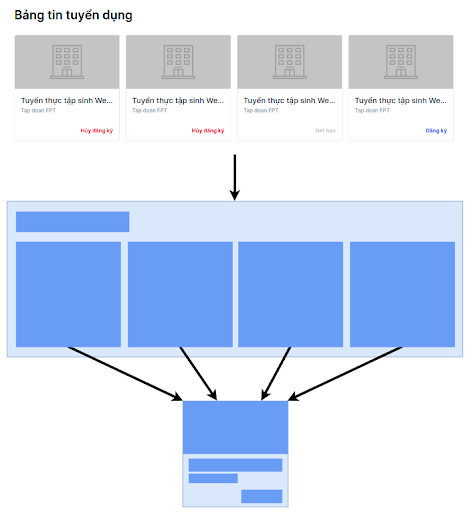
\includegraphics[width=\linewidth]{./images/image34.png}
	\caption{Ví dụ Nguyên lý balance và rhythm ở màn student}
	\label{fig:example_rhythm_syudent}
\end{figure}

Đôi khi việc lặp đi lặp lại các phần tử sẽ gây ra cảm giác nhàm chán, khiến người dùng không biết nên nhìn vào đâu khi truy cập trang web. Để hạn chế điều này thì việc áp dụng nguyên lý hài hòa và thống trị sẽ làm nổi bật dụng ý của trang web, dẫn dắt sự chú ý của người dùng đến với các phần tử cần chú ý. Ví dụ: Trong màn hình trang chủ của sinh viên, phần đăng ký thực tập nằm ở giữa chiếm nửa màn hình, có hình ảnh minh họa khá nổi bật chiếm ngay lấy sự chú ý của người dùng, từ đó hướng sự chú ý sang phần Tìm kiếm tên công ty đang thực tập.

\begin{figure}[H]
	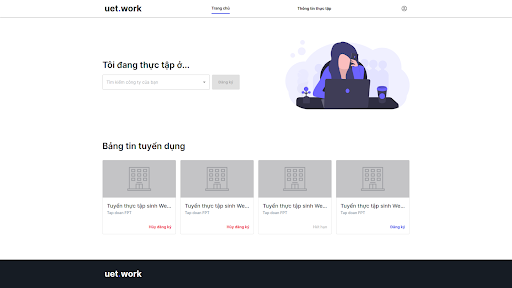
\includegraphics[width=\linewidth]{./images/image35.png}
	\caption{Ví dụ về nguyên lý harmony và dominance}
	\label{fig:example_harmony_dominance}
\end{figure}

\subsection{Thiết kế bảng dữ liệu}

Các màn hình trong hệ thống Quản lý thực tập đa phần đều chứa các bảng dữ liệu. Các bảng này đều được áp dụng từ component DataGrid của thư viện Material UI nên rất đồng đều và có thể tích hợp thêm đầy đủ các tính năng tìm kiếm, lọc, sắp xếp, phân trang phục vụ cho việc quản lý của giảng viên, đối tác và quản trị viên.

\begin{figure}[H]
	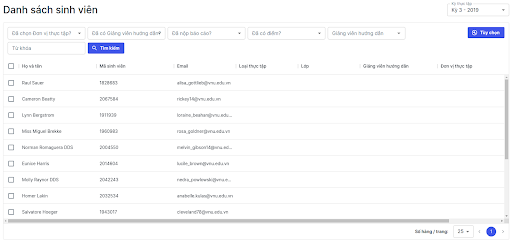
\includegraphics[width=\linewidth]{./images/image36.png}
	\caption{Ví dụ về Bảng dữ liệu}
	\label{fig:example_data_table}
\end{figure}

\end{document}
